%%%%%%%%%%%%%%%%%%%%%%%%%%%%%%%%%%%%%%%%%%%%%%%%%%%%%%%%%%%%%%%%%%%%%%%%%%%%%%%%%%%
% Team:
% Union
% Members: 
% Bernie Huan, Jim Lan, Hoang Tan, Kenny Hsu, Rahul Aditya, Tan Phat, Wei
% Relative files:
% Main.tex, Background_Union.tex, Library.bib, Union_Background_Chart_1.png, Union_Background_Chart_2.png, Union_Background_Chart_3.png, Union_Background_Chart_semi.png, Union_Background_Chart_sup1.png, Union_Background_Chart_sup2.png, Union_Background_Chart_sup3.png, Union_Background_Chart_WSD.png
% Note:
% Do not compile this file compile Main.tex to get the pdf file instead.
%%%%%%%%%%%%%%%%%%%%%%%%%%%%%%%%%%%%%%%%%%%%%%%%%%%%%%%%%%%%%%%%%%%%%%%%%%%%%%%%%%%

\subsection{Automatic creation of metadata}
\textit{\footnotesize Author:Bernie Huan, Jim Lan, Hoang Tan, Kenny Hsu, Rahul Aditya, Tan Phat, Wei.}\\

We are producing a program that automatically generate and extract metadata with natural language processing. 
We also strive to generate XML files with metadata extracted. 
In the best scenario, we will even try to create a search engine together with other groups. 
Also, creating a sutiable interface and structure with some finctions for users is necessary.  
Following discussion is our literature review on natural language processing.

\begin{figure*}[ht]
	\begin{center}
		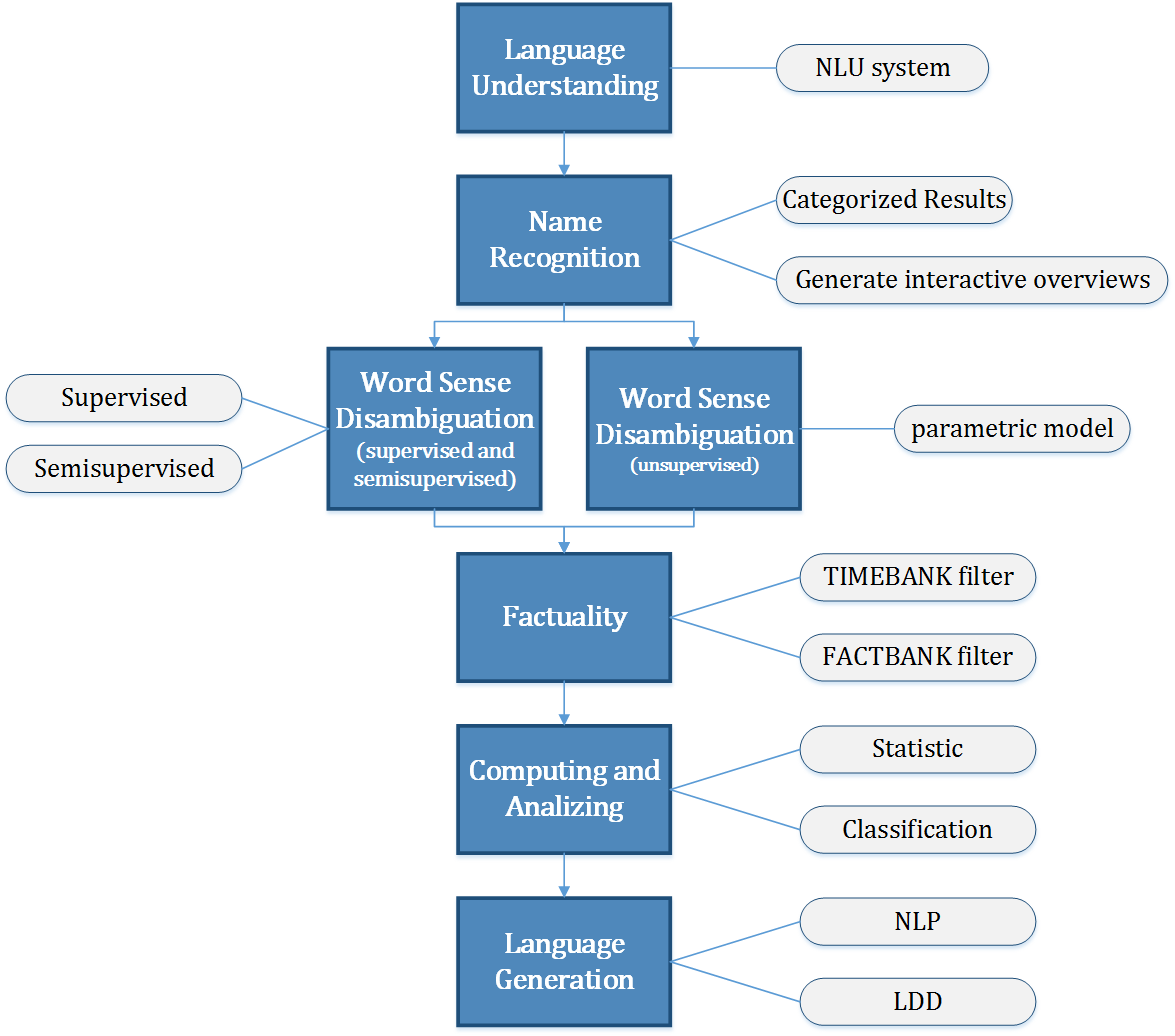
\includegraphics[width=1.8\columnwidth]{Union_Background_Chart_1}
	\end{center}
	\caption{The process of metadata creation.}
\end{figure*}

\subsubsection*{Language understanding}
Natural language understanding (NLU) is a subtopic of natural language processing in artificial intelligence that deals with machine reading comprehension, it's considered an AI-hard problem.

When users search for a sentence, how does the program understand the certain inputs of text? 

We could build a natural language understanding (NLU) system, in which the system's rules for semantic interpretation are 
learnt automatically from training data, which uses a set of possible yes-no questions that can be applied to data items.
After that, it follows rules for selecting the best questions at any node on the basis of training data by using a method for pruning trees to prevent over-training.

\subsubsection*{Name Recognition}

The results could be a country or an animal if users search for the word, Turkey. The meaning is totally different and
definitely make users very confused if he or she is not very familiar with "Turkey". 

There are a lot of misunderstandings like this if users search some words which have multiply meanings.
Sometimes, the results are fully unrelated and this situation is always annoying. 
That would be troublesome when we count frequency of certain words to rank them.

Therefore, it is significantly crucial for a program to totally understand what users want by name recognition in natural language processing. 
The users can find out the results much quicker and will not be confused.

The method to improve the problem above is "categorize the words based on different subjects,topic or genres" by using online database and python program.
Metadata is limited in digital libraries and web resources, try to enlarge them with meaningful, organized and desired
categories \cite{Kules2006}.

Besides dealing with mutiple-meaning words,the most important part of name recognition is to recognize the special names and terms such as locations,people name,country,even company names and academic terms.
Therefore, it is better for search engine to know what user want and huge name corpus are necessary. Plus, this work also can assist previous work.

With above effort,users' exploration and overviews of information could be better supported. 
It will be very convenient to find the results we want and lower the possibility of misunderstandings if users are not 
very familiar with finding the appropriate result in specific fields.\cite{TunThuraThet2010} 
Users dose not have to filter the results which are ranked by browsing frequency popularity. 
Users just can obtain the information and relevance by clicking the specific categories and some reasonable choices.

Plus,creating some choices for users is also vital because this make the searching much more oragnized.
For example,if there are a lot of subtitles such as abstract, introduction,method or references in some standard research 
articles, try to make some choices so that the users can easily find out what they want.
There are a lot of different standard articles in the world.
Making a suitable choices if someone want to creat a personalzed search engine and interface. 
     
Also, users are able to choose multiply fields if the results include a lot of relevant fields. 
That's a big motivation for people to handle this problems. 

A lot of online services have done similar tasks before.
Thus,creating and using an online databasees or automated metadata creation are to be recommended.
The reason is there are many advantages, including integrating with the other cloud services or scaling with what users 
need such as how to categorize the categories.
It is beneficial for people who would like to create a convenient and personalized database or metadata.\\


\subsubsection*{Part-of-speech}

In the English language, we can consider words as the smallest elements that have distinctive meanings.
Based on their uses and functions, words are categorized into several parts of speech, and the 8 major parts of speech in 
English grammar are: noun, pronoun, verb, adverb, adjective, conjunction, preposition, and interjection.
\begin{itemize}
	\item Noun (names)\\
	A word or lexical item denoting any abstract (abstract noun: e.g. home) or concrete entity (concrete noun: e.g. house); a person (doctor, Jim), place (farm, Taiwan), thing (earring, refrigerator), idea (happiness), or quality (ambition). 
	Nouns can also be classified as counted nouns or non-counted nouns; some can belong to any category. 
	The most common part of the speech; they are called naming words.
	
	\item Pronoun (replaces)\\
	A substitute for a noun or noun phrase (e.g. them, he). Pronouns make sentences shorter and clearer since they replace nouns.
	
	\item Adjective (describes, limits)\\
	A modifier of a noun or pronoun (big, brave). 
	Adjectives make the meaning of another word (noun) more precisely.
	
	\item Verb (states action or being)\\
	A word denote an action (walk), occurrence (happen), or state of being (be).
	Without a verb, a group of words cannot be a clause or sentence.
	\item Adverb (describes, limits)\\
	A modifier of an adjective, verb, or other adverb (very, quite). 
	Adverbs make your writing more precisely.
	
	\item Preposition (relates)\\
	A word that relates words to each other in a phrase or a sentence and aids in syntactic context (in, of). 
	Prepositions show the relationship between a noun or a pronoun with another word in a sentence.
	
	\item Conjunction (connects)\\
	A syntactic connector; links words, phrases, or clauses (and, but). 
	Conjunctions connect words or group of words.
	
	\item Interjection (expresses feelings and emotions)\\
	An emotional greeting or exclamation (Huzzah, Alas). 
	Interjections express strong feelings and emotions.
\end{itemize}

\subsubsection*{Part-of-speech tagging}

Part of speech tagging (POS tagging), also called grammatical tagging or word-category disambiguation, which is a process 
of assigning a part of speech to each word in a sentence that based on both definition and its context.\\

\subsubsection*{Word sense disambiguation: supervised and semi-supervised approach}

Word sense disambiguation (WSD) is an open problem of natural language processing and ontology. 
WSD identifies which sense of a word (i.e.meaning) is used in a sentence,
when the word has multiple meanings \cite{Du2013}. 

\begin{figure}[tbh]
	\begin{center}
		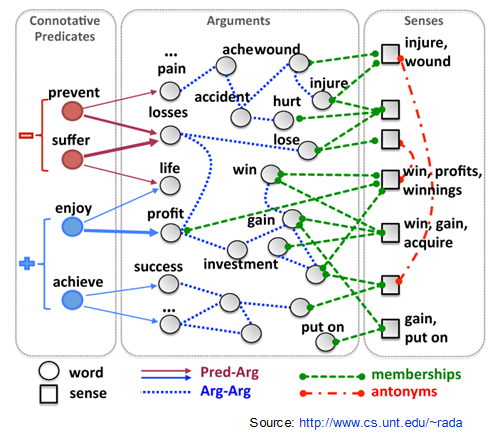
\includegraphics[width=\columnwidth]{Union_Background_Chart_WSD}
	\end{center}
	\caption{GWord+Sense with words and senses. \label{fig1}}
\end{figure}

The solution to this problem impacts other computer-related writing, such as discourse, 
improving relevance of search engines, anaphora resolution, coherence, inference et cetera.

Word Sense Disambiguation(WSD) is related to Natural Language Processing and is also linked with computational languages. 
People introduced it as a solution when they felt the need of some complex problems like machine translation, information retrieval, speech processing and text processing ,etc. 

WSD is mainly focused on determining the sense of word,computationally which is used in a problem by using that word in a particular context. 
Inspite of having a greater number of existing disambiguation algorithms, WSD still has an open problem with the three main parts of the WSD methods being considered by literature: Supervised, Unsupervised and semi-supervised. 

The human brain is quite proficient at word-sense disambiguation. 
The fact that natural language is formed in a way that requires so much of it is a reflection of that neurological reality. 
In other words, human language developed in a way that reflects (and also has helped to shape) the innate ability provided 
by the brain's neural networks. 

In computer science and the information technology that it enables, it has been a long-term challenge to develop the ability 
in computers to do natural language processing and machine learning. 

\subsection*{Supervised}

Supervised methods are based on the assumption that the context can provide enough evidence on its own to disambiguate words. 
Probably every machine learning algorithm going has been applied to WSD, including associated techniques, such as feature selection, parameter optimization, and ensemble learning.

\begin{figure}[tbh]
	\begin{center}
		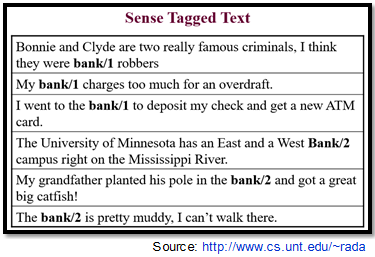
\includegraphics[width=\columnwidth]{Union_Background_Chart_sup1}
	\end{center}
	\caption{Sense tagged text.}
\end{figure}
\begin{figure}[tbh]
	\begin{center}
		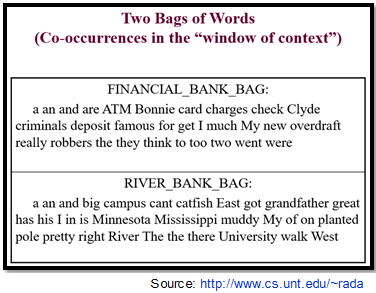
\includegraphics[width=\columnwidth]{Union_Background_Chart_sup2}
	\end{center}
	\caption{Two bags of words(bank).}
\end{figure}
\begin{figure}[tbh]
	\begin{center}
		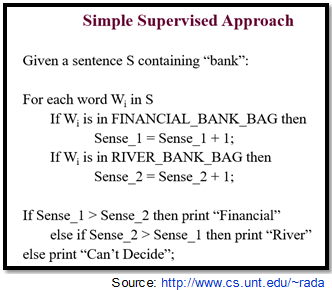
\includegraphics[width=\columnwidth]{Union_Background_Chart_sup3}
	\end{center}
	\caption{Simple Supervised approach.}
\end{figure}

Support Vector Machines and memory-based learning have been shown to be the most successful approaches, to date, probably because they can cope with the high-dimensionality of the feature space. 

However, these supervised methods are subject to a new knowledge acquisition bottleneck since they rely on substantial amounts of manually sense-tagged corpora for training, which are laborious and expensive to create \cite{aramossoto2016onthe}.

\subsubsection*{Semi-supervised}

Because of the lack of training data, many word sense disambiguation algorithms use semi-supervised learning, which allows both labeled and unlabeled data. 
The Yarowsky algorithm was an early example of such an algorithm \cite{Gartner201317}. 
It uses the 'One sense per collocation' and the 'One sense per discourse' properties of human languages for word sense disambiguation. 
Based on observation it has been shown that words tend to exhibit only one sense in most given discourse and in a given collocation. \cite{5599823}

\begin{figure}[tbh]
	\begin{center}
		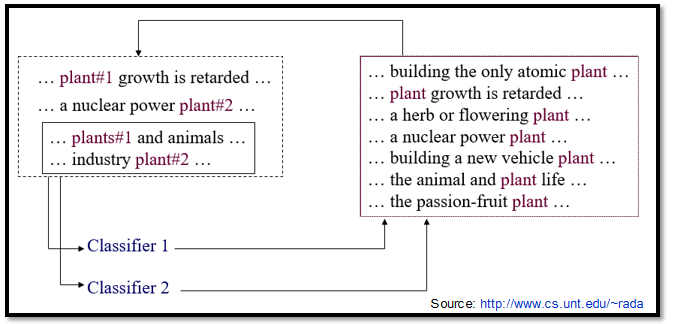
\includegraphics[width=\columnwidth]{Union_Background_Chart_semi}
	\end{center}
	\caption{Classifier that improves over the basic classifier. \label{fig3}}
\end{figure}

The bootstrapping approach starts from a small amount of seed data for each word: either manually tagged training examples or 
a small number of surefire decision rules. 
The seeds are used to train an initial classifier, using any supervised method. This classifier is then used on the untagged portion of the corpus to extract a larger training set, in which only the most confident classifications are included. 
The process repeats, each new classifier being trained on a successively larger training corpus, until the whole corpus is consumed, or until a given maximum number of iterations is reached \cite{Blascheck2016}.

Other semi-supervised techniques use large quantities of untagged corpora to provide co-occurrence information that supplys 
the tagged corpora. 
These techniques have the potential to help in the adaptation of supervised models to different domains.

Also, an ambiguous word in one language is often translated into different words in a second language depending on the sense 
of the word. 
Word-aligned bilingual corpora have been used to infer cross-lingual sense distinctions, a kind of semi-supervised system.\cite{Cheslow2014}

\subsubsection*{Unsupervised}
Unsupervised WSD is the third part of Word sense disambiguation,it has to focus in the sense of the word which is being used 
in a sentence.  
Unsupervised WSD, which relys on single writing can be approached by the use of Naive Bayes' model, which mainly focuses on unsupervised part of the context. 
In this model, a number of sentences are used which contains a particular word which has several meanings. 
The main goal is to divide those words into a specified number of sense groups \cite{4028513}.
The Naive Bayes model applied mathematically entirely focuses on the issue of feature selection, which describes its two types:

\begin{enumerate}
	\item Pedersen and Bruce local type features.
	\item WordNet-based feature selection.
\end{enumerate}

\begin{enumerate}
	\item Pedersen and Bruce local type features:
\end{enumerate}
Three different feature sets have been used by 'Pedersen and Bruce' (under Naive Bayes model) for each word to formulate such 
a model describing the distributions of sense groups of that word in Unsupervised WSD.

Features which were taken into account are:
\textbf{Morphology:} The pattern of word formation in a particular language is called as Morphology.
This feature represents the morphology \cite{5494927} of the ambiguous word and is denoted by M. 
In case of nouns, M acts as Binary which indicates whether the word is plural or singular.
For verbs, M indicates the tense of the verb and can have up to seven possible values.
This feature is not applicable for adjectives.

\textbf{Part-of-speech:} This feature represents the part-of-speech \cite{6982457} of the word and tells the position of the ambiguous word.
Each POS feature can have one of five possible values: noun, verb, adjective, adverb or other.

\textbf{Co-occurences:} This feature also acts as binary variables representing whether the most frequent content word in all the sentences contain the ambiguous word can occur anywhere in the sentence or not.

\begin{enumerate}
	\item WordNet-based feature selection:
\end{enumerate}
WordNet is a large lexical database of English. 
The approach to WSD relies on a set of features formed by the actual words occuring near the target word and 
reduces the size of this feature set by performing knowledge-based feature selection that relies entirely on WordNet.
The WN semantic network provides the words considered relevant for the set of senses taken into consideration corresponding 
to the target word.

In WordNet, noun is the most developed portion as per the research done over the performance for knowledge-based disambiguation.
For adjectives, the same disambiguation method has taken into account as the similarity relation, which  is typical of this 
part of speech.
Verbs are suggested to use additionally whenever possible.
As a result of using only those words indicated as being relevant and recommended by WordNet, a much small vocabulary was obtained.
Therefore, a much smaller number of features were taking part in the disambiguation process.

So, this background focuses mainly on the issues of feature selection for unsupervised WSD performed with an underlying Naive Bayes model.
\todo{Really? This section is shorter.}

The difference between 'Supervised' and 'Unsupervised' WSD is:

\begin{enumerate}
	\item The Supervised WSD approach requires a large amount of data in order to achieve a reliable result and generally the scope is limited to some words. 
	Whereas the Unsupervised WSD approach does not use any corpus and suggests the suitable information extracted to the word knowledge base.
	This method is used in case of performing WSD without data learning.
	\item The Supervised approaches make use of information from labeled training data while the Unsupervised does not depend upon any labeled data, it uses a multi-lingual thesaurus that contains millions of biomedical and health related concepts, their synonymous names and their relationships.
\end{enumerate}

\todo[inline]{A summary on list format can be motivated, but then each item need to be brief and you should not introduce anything new like UMLS in it.}

\subsubsection*{Factuality}

In the process of producing metadata, which should be the most precise information and representing the text, validity of such metadata must be checked. 
Therefore tools for fact checks are developed based on linguistic techniques. 

The tool could detect facts and excludes authors' subjective opinions \cite{Agerri2014}. 
From the authors's perspective, the two main set of tools having such functions is TIMEBANK and FACTBANK.(yes, the authors used capitalized name)

TIMEBANK was first proposed in \cite{pustejovsky2003timebank}. 
The idea was based on that English language has different tenses which could be exploited as signals for fact check. 
An example below could help to clarify the ideas.
 Let's examine these sentences:

\begin{itemize}
	\item I will go to Chimei museum tomorrow.
	\item Chimei museum is near Tainan District.
	\item I was in UK in 2012.
\end{itemize}

The first sentence is simple future tense which implies something has never actually happened, the second sentence is simple present tense which can directly imply facts,and the last sentence is in simple past tense which is about something already happened (which is facts),but is no longer a fact right now, so such fact must be used with caution. 

The reason for introducing such tool is that even scientific research articles can be glittering with subjective comments, opinions or even assumption from authors \cite{schultze2000confessional}. 
In addition to TIMEBANK, many other tools can be another filter for fact extraction. 
\cite{Dave2003mining} Identify words, clauses and phrases that show emotional state of the authors. 

The choice in expression of facts could also be a helpful indicator to show whether authors are subjectively supporting a cause, an opinion and so on \cite{Wiebe2005}. 
Among these mentioned approaches, this paper highly favors creation a kind of thesaurus compiled of linguistic signaling for non-factually statements such as FACTBANK,which is built by \cite{Sauri2009}. 
Following example shows how subjective statements can be picked out.

\begin{itemize}
	\item Channelization would guarantee high flow velocity in rivers, flooding and consequent degradation of riparian community (1a).
	\item Funding agencies would be happy with big entrepreneurs, instead of small and medium enterprises (1b).
	\item Tolerance to dictatorship would has negative influences on anarchist movement (2a).
	\item Tolerance to dictatorship would doom anarchist movement (2b).
\end{itemize}

It is easy to find in statement (1a) is an absolute fact. 
Statement (1b) is however affected by emotional state of authors. 
After re-writing (1b) into: Funding agencies lend more money with lower interest rate to big entrepreneurs, instead of small 
and medium enterprises,sentence (1b) become a face-based statement. 
In another case, statement (2a) is a fact-based statement while in statement (2b), authors are stressing their dislike toward dictatorship.

Fact checks in language generation is a new field but many useful tools have been developed. 
Each of them has their own function and could complement each others. 
In the limit of this study, we are using both of TIMEBANK and FACTBANK together for fact check.



\subsubsection*{Language generation}

Natural language generation (NLG) is one branch of natural language processing. 
The goal is generating the words that human being uses via machine automatically. 
In order to use this technique, six basic activities are done: 
\begin{enumerate}
	\item content determination: In this active, we create some messages which are communicated in the text. 
	These messages shall be labeled and the entity in the messeges is also distinguished, which is convenient for us to 
	use these data within the following step.
	\item discourse planning: This part is closely related to the previous part. 
	We determine the order and the structure of the messeges.
	\item sentence aggregation:This part combines several messeges into sentences. 
	Although some of messeges have been a sentence, we can improve the influency of messeges by combining them.
	\item lexicalization: This part make the messege more precise by use the specific words and concepts. 
	Then people can get the ideas of the messeges more quickly.
	\item referring expression generation: This part is a litte same as the previous part. 
	But the difference is that this part differentiate the one domain to the other domains.
	\item linguistic realization: Last part is to make the expression follow the rules of grammer, part of speech and the natural language rule.
\end{enumerate}
\cite{aramossoto2016onthe}.\todo{Where? Please explain the 6 terms. What are they?} 
The advantage of this technique is that it is flexible, since there is no standardization. 
But it also has the difficulty in the implication of this technique.\cite{aramossoto2016onthe}No standardization means that 
no rules can be followed. 

Without logic method, it is almost impossible to code and be realized by computer.
Thus, the another concept is proposed. This way has the logical method, also the algorithm is easy to realize.
The technique is linguistic discription of data.
\todo{Now you jump too far. More explanations are needed.}
Linguistic description of data (LDD) is a concept that applied the fuzzy set theory in the linguistic field. 
At the beginning, comparing to the NLG field, it is a newer technique to solve the problem of language generation. 
However, the basic steps of LDD have been built. 
The four main parts in this technique are inputing data, linguistic variable, fuzzy quantifiers and evaluation criteria \cite{aramossoto2016onthe}. 
Some of them are similar to the concept. 
The advantage of this technique is that it has been implied in many fields just like weather forecast \cite{Ramos-SotoBBT14}. 
Also, many practical methods have been proposed. 
However, it still has a long way to go.

These two techniques are usually combined together nowadays. 
The concept of NLG and the practical approach of LDD could be used in the same time to provide the better performance in language generate field.
\subsection*{API}
In most procedural languages, an API specifies a set of functions or routines that accomplishes a specific task, or are allowed to interact with a specific software component. 
This specification is presented in a human readable format in paper books or in electronic formats like eBooks or as man pages. For example, the math API on Unix systems is a specification on how to use the mathematical functions included in the math library. 
Among these functions there is a function named sqrt(), that can be used to compute the square root of a given number.

The Unix command man 3 sqrt presents the signature of the function sqrt in the form:

SYNOPSIS
#include <math.h>
double sqrt(double X);
float  sqrtf(float X);
DESCRIPTION
sqrt computes the positive square root of the argument. ...
RETURNS
On success, the square root is returned. If X is real and positive...
This description mean that sqrt() function returns the square root of a positive floating point number (single or double precision), as another floating point number. 
The main page also states that the calling program must include the math.h header file to be able to reference the functions present in the math library.

Hence the API in this case can be interpreted as the collection of the include files used by a program, written in the C language, to reference that library function, and its human readable description provided by the man pages.

Similarly, other languages have procedural libraries; for example, Perl has dedicated APIs for the same mathematical task with built-in documentation available, which is accessible using the perldoc utility:

$ perldoc -f sqrt
sqrt EXPR
sqrt    #Return the square root of EXPR.  If EXPR is omitted, returns
#square root of $_.  Only works on non-negative operands, unless
#you've loaded the standard Math::Complex module.
API in object-oriented languages[edit]
In its simplest form, an object API is a description of how objects work in a given object-oriented language – usually it is expressed as a set of classes with an associated list of class methods.

For example, in Java, if the class Scanner is to be used (a class that reads input from the user in text-based programs), it is necessary to import the java.util.Scanner library. 
Then objects of type Scanner can be used by invoking some of the class' methods:

import java.util.Scanner;

public class Test {
	public static void main(String[] args) {
		System.out.println("Enter your name:");
		Scanner inputScanner = new Scanner(System.in);
		String name = inputScanner.nextLine();
		System.out.println("Your name is " + name + ".");
		inputScanner.close();
	}
}
In the example above, methods nextLine() and close() are part of the API for the Scanner class, and hence are described in the documentation for that API, e.g.:

public String nextLine()

Advances this scanner past the current line and returns the skipped input...

Returns:

the line that was skipped

Throws:

NoSuchElementException - if no line found

IllegalStateException - if this scanner is closed

More generally, in object-oriented languages, an API usually includes a description of a set of class definitions, with a set of behaviors associated with those classes. 
This abstract concept is associated with the real functionality exposed, or made available, by the classes that are implemented in terms of class methods (or more generally by all its public components hence all public methods, but also possibly including any internal entity made public like: fields, constants, nested objects, enums, etc.).

The API in this case can be conceived of as the totality of all the methods publicly exposed by the classes (usually called the class interface). 
This means that the API prescribes the methods by which one interacts with/handles the objects derived from the class definitions.

More generally, one can see the API as the collection of all the kinds of objects one can derive from the class definitions, and their associated possible behaviors. 
Again: the use is mediated by the public methods, but in this interpretation, the methods are seen as a technical detail of how the behavior is implemented.

For instance: a class representing a Stack can simply expose publicly two methods push() (to add a new item to the stack), and pop() (to extract the last item, ideally placed on top of the stack).

In this case the API can be interpreted as the two methods pop() and push(), or, more generally, as the idea that one can use an item of type Stack that implements the behavior of a stack: a pile exposing its top to add/remove elements. 
The second interpretation appears more appropriate in the spirit of object orientation.

This concept can be carried to the point where a class interface in an API has no methods at all, but only behaviors associated with it.
 For instance, the Java and Lisp language APIs include the interface named Serializable, which is a marker interface that requires each class implementing it to behave in a serialized fashion. 
 This does not require implementation of a public method, but rather requires any class that implements this interface to be based on a representation that can be saved (serialized) at any time.

Similarly the behavior of an object in a concurrent (multi-threaded) environment is not necessarily determined by specific methods, belonging to the interface implemented, but still belongs to the API for that Class of objects, and should be described in the documentation.[5]

In this sense, in object-oriented languages, the API defines a set of object behaviors, possibly mediated by a set of class methods.

In such languages, the API is still distributed as a library. For example, the Java language libraries include a set of APIs that are provided in the form of the JDK used by the developers to build new Java programs. 
The JDK includes the documentation of the API in JavaDoc notation.

The quality of the documentation associated with an API is often a factor determining its success in terms of ease of use.

API libraries and frameworks[edit]
An API is usually related to a software library: the API describes and prescribes the expected behavior while the library is an actual implementation of this set of rules.
 A single API can have multiple implementation (or none, being abstract) in the form of different libraries that share the same programming interface.

An API can also be related to a software framework: a framework can be based on several libraries implementing several APIs, but unlike the normal use of an API, the access to the behavior built into the framework is mediated by extending its content with new classes plugged into the framework itself. 
Moreover, the overall program flow of control can be out of the control of the caller, and in the hands of the framework via inversion of control or a similar mechanism.[6][7]

API and protocols[edit]
An API can also be an implementation of a protocol.

When an API implements a protocol it can be based on proxy methods for remote invocations that underneath rely on the communication protocol. The role of the API can be exactly to hide the detail of the transport protocol.
 E.g.: RMI is an API that implements the JRMP protocol or the IIOP as RMI-IIOP.

Protocols are usually shared between different technologies (system based on given computer programming languages in a given operating system) and usually allow the different technologies to exchange information, acting as an abstraction/mediation level between the two different environments. 
Protocol hence can be considered remote APIs, local APIs instead are usually specific to a given technology: hence an API for a given language cannot be used in other languages, unless the function calls are wrapped with specific adaptation libraries.

To enable the exchange of information among systems that use different technologies, when an API implements a protocol, it can prescribe a language-neutral message format: e.g. SOAP uses XML as a general container for the messages to be exchanged, similarly REST API can use both XML and JSON.

Object exchange API and protocols[edit]
An object API can prescribe a specific object exchange format that a program can use locally within an application, while an object exchange protocol can define a way to transfer the same kind of information in a message sent to a remote system.

When a message is exchanged via a protocol between two different platforms using objects on both sides, the object in a programming language can be transformed (marshalled and unmarshalled[8]) in an object in a remote and different language: so, e.g., a program written in Java invokes a service via SOAP or IIOP written in C# both programs use APIs for remote invocation (each locally to the machine where they are working) to (remotely) exchange information that they both convert from/to an object in local memory.

Instead when a similar object is exchanged via an API local to a single machine the object is effectively exchanged (or a reference to it) in memory: e.g. via memory allocated by a single process, or among multiple processes using shared memory, an application server, or other sharing technologies like tuple spaces.

Object remoting API and protocols[edit]
An object remoting API is based on a remoting protocol, such as CORBA, that allows remote object method invocation.
 A method call, executed locally on a proxy object, invokes the corresponding method on the remote object, using the remoting protocol, and acquires the result to be used locally as return value.[9]

When remoting is in place, a modification on the proxy object corresponds to a modification on the remote object.
When only an object transfer takes place, the modification to the local copy of the object is not reflected on the original object, unless the object is sent back to the sending system.

API sharing and reuse via virtual machine[edit]
Some languages like those running in a virtual machine (e.g. .NET CLI compliant languages in the Common Language Run time (CLR), and JVM compliant languages in the Java Virtual Machine) can share an API. 
In this case, a virtual machine enables language interoperability, by abstracting a programming language using an intermediate byte code and its language bindings.
 In these languages, the compiler performs just-in-time compilation or ahead-of-time compilation transforming the source code, possibly written in multiple languages, into its language-independent byte code representation.

For instance, through the byte code representation, a program written in Groovy or Scala language can use any standard Java class and hence any Java API. 
This is possible thanks to the fact both Groovy and Scala have an object model that is a super set of that of the Java language; thus, any API exposed via a Java object is accessible via Groovy or Scala by an equivalent object invocation translated in byte code.

On the other side, Groovy and Scala introduce first-class entities that are not present in Java, like closures. 
These entities cannot be natively represented in Java language (Java 8 introduced the concept of lambda expression); thus, to enable inter operation, a closure is encapsulated in a standard Java object. 
In this case the closure invocation is mediated by a method named call(), which is always present in an closure object as seen by Java, and in Java the closure does not represent a first-class entity.

Web APIs
Main article: Web API
Web APIs are the defined interfaces through which interactions happen between an enterprise and applications that use its assets.
An API approach is an architectural approach that revolves around providing programmable interfaces to a set of services to different applications serving different types of consumers.[10] When used in the context of web development, an API is typically defined as a set of Hypertext Transfer Protocol (HTTP) request messages, along with a definition of the structure of response messages, which is usually in an Extensible Markup Language (XML) or JavaScript Object Notation (JSON) format. 
While "web API" historically has been virtually synonymous for web service, the recent trend (so-called Web 2.0) has been moving away from Simple Object Access Protocol (SOAP) based web services and service-oriented architecture (SOA) towards more direct representational state transfer (REST) style web resources and resource-oriented architecture (ROA).
 Part of this trend is related to the Semantic Web movement toward Resource Description Framework (RDF), a concept to promote web-based ontology engineering technologies. Web APIs allow the combination of multiple APIs into new applications known as mashups.

Web use to share content
The practice of publishing APIs has allowed web communities to create an open architecture for sharing content and data between communities and applications. 
In this way, content that is created in one place can be dynamically posted and updated in multiple locations on the web:

Photos can be shared from sites like Flickr and Photobucket to social network sites like Facebook and MySpace.
Content can be embedded, e.g. embedding a presentation from SlideShare on a LinkedIn profile.

Content can be dynamically posted. 
Sharing live comments made on Twitter with a Facebook account, for example, is enabled by their APIs.
Video content can be embedded on sites served by another host.
User information can be shared from web communities to outside applications, delivering new functionality to the web community that shares its user data via an open API. One of the best examples of this is the Facebook Application platform. 
Another is the Open Social platform.
If content is a direct representation of the physical world (e.g., temperature at a geospatial location on earth) then an API can be considered an "Environmental Programming Interface" (EPI). 
EPIs are characterized by their ability to provide a means for universally sequencing events sufficient to utilize real-world data for decision making.
Implementations
The POSIX standard defines an API that allows writing a wide range of common computing functions in a way such that they can operate on many different systems (Mac OS X, and various Berkeley Software Distributions (BSDs) implement this interface).
However, using this requires re-compiling for each platform. A compatible API, on the other hand, allows compiled object code to function with no changes to the system that implements that API. This is beneficial to both software providers (where they may distribute existing software on new systems without producing and →distributing upgrades) and users (where they may install older software on their new systems without purchasing upgrades), although this generally requires that various software libraries implement the necessary APIs as well.

Microsoft has shown a strong commitment to a backward compatible API, particularly within their Windows API (Win32) library, such that older applications may run on newer versions of Windows using an executable-specific setting called "Compatibility Mode".

Among Unix-like operating systems, there are many related but incompatible operating systems running on a common hardware platform (particularly Intel 80386-compatible systems). 
There have been several attempts to standardize the API such that software vendors may distribute one binary application for all these systems; however, to date, none of these has met with much success. 
The Linux Standard Base is attempting to do this for the Linux platform, while many of the BSD Unixes, such as FreeBSD, NetBSD, and OpenBSD, implement various levels of API compatibility for both backward compatibility (allowing programs written for older versions to run on newer distributions of the system) and cross-platform compatibility (allowing execution of foreign code without recompiling).

API design[edit]
Several principles are commonly used to govern the process of designing APIs.
 Parnas proposed the concept of information hiding in 1972. The principle of information hiding is that one may divide software into modules, each of which has a specified interface. 
 The interfaces hide the implementation details of the modules so that users of modules need not understand the complexities inside the modules. 
 These interfaces are APIs, and as a result, APIs should expose only those module details that clients must know to use modules effectively. 
 Software architecture is dedicated to creating and maintaining high-level software structures—which typically includes modules. 
 APIs reflect interfaces between modules. Thus, a system architecture is inextricably related to the APIs that express that architecture. However, many decisions involved in creating APIs are not architectural, such as naming conventions and many details on how interfaces are structured.

These details of how interfaces are structured, as well as the software architecture, have significant impacts on software quality. 
For example, Cataldo et al. found that bugginess is correlated with logical and data dependencies in software.
This implies that to reduce bug rates, software developers should carefully consider API dependencies.

Conway's Law states that the structure of a system inevitably reflects the structure of the organization that created it. 
This suggests that to understand how APIs are designed in the real world, one must also understand the structures of software engineering organizations.
 Likewise, an API group should structure itself according to what the API needs. 
 In a study of 775 Microsoft software engineers, Begel et al. found that in addition to coordinating regarding API design, software engineers even more commonly coordinate regarding schedules and features.
 This reinforces the view that software organizations collaborate extensively and that organizational structure is important.

Several authors have created recommendations for how to design APIs, such as Joshua Bloch, Kin Lane, and Michi Henning. 
Since one of the principles of API design is that an API should be consistent with other APIs already in use in the system, the details of API design are somewhat language- and system-dependent.

Release policies[edit]
The main policies for releasing an API are:

Protecting information on APIs from the general public.
 For example, Sony used to make its official PlayStation 2 API available only to licensed PlayStation developers. 
 This enabled Sony to control who wrote PlayStation 2 games. 
 This gives companies quality control privileges and can provide them with potential licensing revenue streams.
Making APIs freely available.
 For example, Microsoft makes the Microsoft Windows API public, and Apple releases its APIs Carbon and Cocoa, so that software can be written for their platforms.
A mix of the two behaviors can be used as well.

Public API implications[edit]
An API can be developed for a restricted group of users, or it can be released to the public.

An important factor when an API becomes public is its interface stability. 
Changes by a developer to a part of it—for example adding new parameters to a function call—could break compatibility with clients that depend on that API.

When parts of a publicly presented API are subject to change and thus not stable, such parts of a particular API should be explicitly documented as unstable. 
For example, in the Google Guava library the parts that are considered unstable, and that might change in a near future, are marked with the Java annotation @Beta.

API deprecation[edit]
A public API can sometimes declare parts of itself as deprecated. 
This usually means that such part of an API should be considered candidates for being removed, or modified in a backward incompatible way.

When adopting a third-party public API, developers should consider the deprecation policy used by the producer of that API; 
if a developer publicly releases a solution based on an API that becomes deprecated, he/she might be unable to guarantee the provided service.

API documentation[edit]

This section does not cite any sources. Please help improve this section by adding citations to reliable sources.
 Unsourced material may be challenged and removed. (April 2015) (Learn how and when to remove this template message)

Professional-level documentation for an API should strive to include the following parts:

Reference documentation 
A description of the functions and objects in the API (see the subsection API reference documentation)
Overview and concepts 
A narrative description of the different parts of the API and how they interact. 
Major frameworks in the API, such as its GUI, network, and file system frameworks should have their own separate section.
Tutorials/training classes 
Step-by-step instructions that show developers how to accomplish a particular task. 
The text should include code that developers can copy into their own applications. For example, a training class for a cryptographic API would include code that shows developers how to use the API to encrypt a file.
Installation/getting started/troubleshooting documentation 
One or more documents that show developers how to do the following:
Obtain the software development kit (SDK) for the API
Install the SDK on a development machine
Obtain keys, accounts, and so forth that allow access
Deploy or provide client libraries
Troubleshoot problems with using the SDK
SDK tools documentation 
Documents that describe how to install and use build, compile, and deploy tools
License information 
Documents that describe the API license
API reference documentation[edit]
The reference documentation for an API is an intrinsic part of any API, and without it the API is unusable. Every aspect of the API, no matter how trivial, should be stated explicitly.

When an API documents a library of functions in a procedural language, it should include:

a description of all the data structures it depends upon
a description of all the functions signatures, including:
function names
function parameters names (when it applies) and types
return type for the functions
for each parameter if the parameter is possibly subjected to modification inside the function
a description of the handling of any error condition
pre- and post-conditions or invariants
more generally how the state has changed after the function execution
possible side-effects
any accessibility or visibility constraint.
An object API should document:

the relationship of any type to other types: inheritance (super-types, sub-types, implemented interfaces or traits), composite structures, delegating entities or any mixed-in set of functionality
the public part of an object derived from a class definition, hence:
its public constants
the name and type of the member variables (fields or properties) that are directly accessible for any object
the signature of the class methods including information similar to that for functions in procedural languages, possibly including a list of getter and setter methods used to access or modify encapsulated information
any class-specific operators, in case the language supports operator overloading
indication whether the fields or methods have a static nature
any constraint that applies to the objects one can create
nested structures, like inner classes or enumerations.
An API in a language using exception handling should report any kind of exception possibly thrown and the specific condition that can cause them to happen.

An API that can be used in a concurrent environment should include indications on how its behavior changes due to possible concurrent access to it: general usability in a concurrent context and possible race conditions.

An API with unstable parts should document them as unstable.

An API with deprecated parts should document them as deprecated.

An API that implements a communications protocol should indicate its general behavior, and should detail:

How to set up a communication session based on that protocol, and prerequisites for correctly setting up a communication session
If the communication is stateful or stateless
In case of stateful sessions: how to handle the state
The notation for the kind of messages the protocol can transport
How the protocol handles communication errors
If, in case of communication errors, the protocol can resubmit a message
Security levels supported, and how to secure communication
Authentication required to set up a session
If the communication can be associated to a transactional processing, and consequently how to handle transactions
If the communication can be embedded in an extended conversation, and consequently how to handle the conversation
A graphical API should document:

Graphical elements it can handle
How to render graphical elements
How to lay out elements on the graphical canvas, and how to compose them
How to interact with graphical elements
How to handle user input, e.g.,
How to add callback to specific user events
How to read information from input fields
An API that interacts with a device should document how to:

Access the device to extract data from it
Modify the state of the device, when possible
Detect error conditions in the device.
An API should always indicate, where applicable:

Language version number
Library and other resource dependencies
Protocol versions it is compatible with or that it implements
Operating system or platform version it supports
An API that can be used in multiple languages via some form of language inter-operation should document any restrictions to its use by languages other than its native language.

API documentation can be enriched with metadata information: like Java annotation, or CLI metadata. This metadata can be used by the compiler, tools, and by the run-time environment to implement custom behaviors or custom handling.

APIs and copyrights[edit]
Ambox current red.svg
This article is outdated. Please update this article to reflect recent events or newly available information. (August 2015)
Main article: Oracle America, Inc. v. Google, Inc.
In 2010, Oracle Corporation sued Google for having distributed a new implementation of Java embedded in the Android operating system.
 Google had not acquired any permission to reproduce the Java API, although a similar permission had been given to the OpenJDK project. 
 Judge William Alsup ruled in the Oracle v. Google case that APIs cannot be copyrighted in the U.S, and that a victory for Oracle would have widely expanded copyright protection and allowed the copyrighting of simple software commands:

To accept Oracle's claim would be to allow anyone to copyright one version of code to carry out a system of commands and thereby bar all others from writing their own different versions to carry out all or part of the same commands.

In 2014, however, Alsup's ruling was overturned on appeal, though the question of whether such use of APIs constitutes fair use was left unresolved.

API examples[edit]
See also: Category:Application programming interfaces
ASPI for SCSI device interfacing
Cocoa and Carbon for the Macintosh
DirectX for Microsoft Windows
EHLLAPI
Java APIs
ODBC for Microsoft Windows
OpenAL cross-platform sound API
OpenCL cross-platform API for general-purpose computing for CPUs & GPUs
OpenGL cross-platform graphics API
OpenMP API that supports multi-platform shared memory multiprocessing programming in C, C++ and Fortran on many architectures, including Unix and Microsoft Windows platforms.
Server Application Programming Interface (SAPI)
Simple DirectMedia Layer (SDL)
Language bindings and interface generators[edit]
APIs that are intended to be used by more than one high-level programming language often provide, or are augmented with, facilities to automatically map the API to features (syntactic or semantic) that are more natural in those languages. 
This is known as language binding, and is itself an API. The aim is to encapsulate most of the required functionality of the API, leaving a "thin" layer appropriate to each language.

Below are listed some interface generator tools that bind languages to APIs at compile time:

SWIG – an open-source interfaces bindings generator supporting numerous programming languages
F2PY – a Fortran to Python interface generator
\newpage % Ends the current page and causes all figures and tables to be printed